% (c)~2014 Claudio Carboncini - claudio.carboncini@gmail.com
% (c)~2014 Dimitrios Vrettos - d.vrettos@gmail.com
\section{Esercizi}
\subsection{Esercizi dei singoli paragrafi}
\subsection*{4.1 - Risoluzione delle disequazioni di secondo grado}

\begin{esercizio}[\Ast]
 \label{ese:4.1}
Risolvi le seguenti disequazioni di secondo grado con il metodo algebrico.
\begin{multicols}{3}
 \begin{enumeratea}
 \item~$x^2-6x\le 0$;
 \item~$5x^2>0$;
 \item~$x^2+x>0$;
 \item~$x^2\le 0$;
 \item~$3x^2\le -1$;
 \item~$x^2-9>0$;
 \item~$2x^2-3x+1>0$;
 \item~$-x^2+3x\ge 0$;
 \item~$3x^2+x-2>0$;
 \item~$x^2-4>0$;
 \item~$\frac 4 3x^2-\frac 1 3x-1<0$;
 \item~$x^2-8\le 0$.
 \end{enumeratea}
 \end{multicols}
\end{esercizio}

\begin{esercizio}[\Ast]
 \label{ese:4.2}
Risolvi le seguenti disequazioni di secondo grado con il metodo algebrico.
\begin{multicols}{3}
 \begin{enumeratea}
 \item~$x^2-5x+3\ge 0$;
 \item~$x^2-4x+9>0$;
 \item~$x^2-6x+8\le 0$;
 \item~$x^2+3x-4\ge 0$;
 \item~$x^2-4x-9\le 0$;
 \item~$x^2-9x+18<0$;
 \item~$x^2-8x+15\ge 0$;
 \item~$-2x^2\ge 0$;
 \item~$3x^2-\frac 2 3x-1\le 0$;
 \item~$x^2+5>0$;
 \item~$x^2+6x-2>0$;
 \item~$2x^2+5x+4\le 0$.
 \end{enumeratea}
 \end{multicols}
\end{esercizio}

\begin{esercizio}[\Ast]
\label{ese:4.3}
Risolvi le seguenti disequazioni di secondo grado con il metodo algebrico.
\begin{multicols}{3}
 \begin{enumeratea}
 \item~$x^2-3x-\frac 5 2<0$;
 \item~$x^2+1>0$;
 \item~$-x^2+5\le 0$;
 \item~$x^2+x\ge 0$;
 \item~$(x+1)^2\ge 0$;
 \item~$x^2>1$;
 \item~$2x^2-6<0$;
 \item~$-x^2-1\le 0$;
 \item $-(x-1)^{2}\le 0$.
 \end{enumeratea}
 \end{multicols}
\end{esercizio}

\begin{esercizio}[\Ast]
\label{ese:4.4}
Risolvi le seguenti disequazioni di secondo grado con il metodo algebrico.
\begin{multicols}{3}
 \begin{enumeratea}
 \item~$x^2+1<1$;
 \item~$x^2-8X+16>0$;
 \item~$\frac{x^{2}}{2}+4x+8>0$;
 \item~$\frac{x^{2}}{3}-x-\frac{4}{3}<0$;
 \item~$x^2-8x+15<0$;
 \item~$2x^2-3x-2>0$.
 \end{enumeratea}
 \end{multicols}
\end{esercizio}

\begin{esercizio}[\Ast]
\label{ese:4.5}
Risolvi le seguenti disequazioni di secondo grado con il metodo algebrico.
\begin{multicols}{3}
 \begin{enumeratea}
 \item~$-3x^2+x+\frac 1 4<0$;
 \item~$3x^2-2x-1>0$;
 \item~$\frac{x^{2}}{5}-2x+5<0$;
 \item~$x^2+3x+8>0$;
 \item~$x^2-2x\ge 0$;
 \item~$-5x^2+4x+1\le 0$.
 \end{enumeratea}
 \end{multicols}
\end{esercizio}

\subsection*{4.2 - Risoluzione grafica di una disequazione di secondo grado}

\begin{esercizio}
 \label{ese:4.6}
Rappresentare nel riferimento cartesiano ortogonale le seguenti parabole.
\begin{multicols}{2}
 \begin{enumeratea}
 \item~$ y=-3x^2+x $;
 \item~$ y=\frac 1 2x-2x+\frac 3 2 $;
 \item~$ y=x^2+x-1 $;
 \item~$ y=x^2-x+1 $.
 \end{enumeratea}
 \end{multicols}
\end{esercizio}

\begin{esercizio}
 \label{ese:4.7}
Rappresentare nel riferimento cartesiano ortogonale le seguenti parabole.
\begin{multicols}{2}
 \begin{enumeratea}
 \item~$ y=-3x^2+3 $;
 \item~$ y=x^2+4x+3 $;
 \item~$ y=x^2+\frac 3 5 $;
 \item~$ y=-\frac 2 5x^2+4x-\frac 1 5 $.
% \item~$ y=-\frac 1 2 x^2-4x-1 $.
 \end{enumeratea}
 \end{multicols}
\end{esercizio}

\begin{esercizio}
 \label{ese:4.8}
Per ciascun grafico di parabola $y=ax^2+bx+c$ indica il segno del primo coefficiente e del discriminante, la natura dei suoi zeri (reali distinti, reali coincidenti, non reali), il segno della funzione.
\begin{center}
 % (c) 2012 Dimitrios Vrettos - d.vrettos@gmail.com
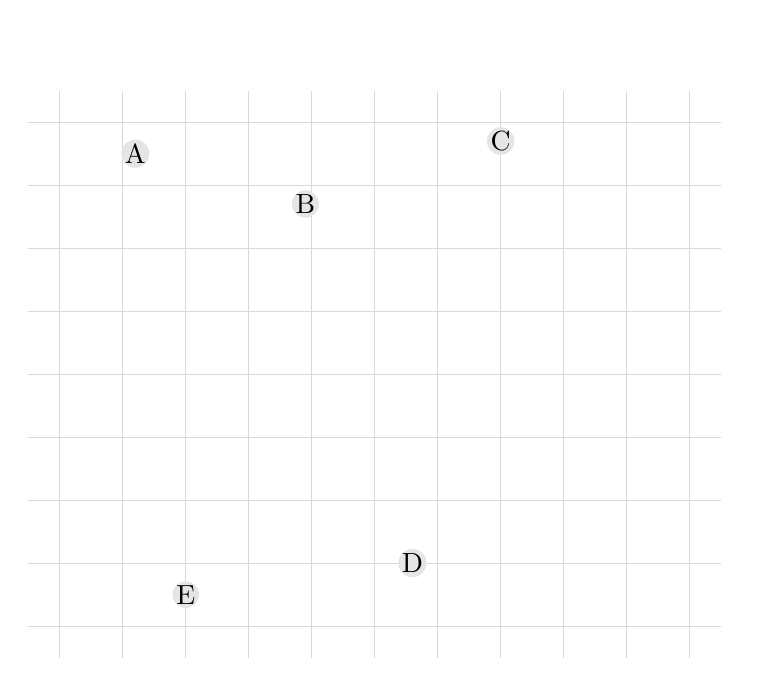
\begin{tikzpicture}[x=8mm, y=8mm]
\draw[step=0.8cm,color=gray!30] (-5.5,-4.5) grid (5.5,4.5);
  \tkzInit[xmin=-5,xmax=5,ymin=-4.5,ymax=4.5]
  \clip (-5.5,-4.5) rectangle (6,5.5);
  \begin{scope}[font=\small]
    \tkzAxeY[orig = false, label options={left = 1pt}]
    \tkzAxeX[orig = true, label options={below = 1pt}]
  \end{scope}
  \tkzFct[domain=-1.5:1.5,thick,color=darkgray]{2*x*x-1}
  \node [inner sep=0pt, circle, fill=gray!20] (a) at (-1.1, 2.7) {B};
  \tkzFct[domain=0:3,thick,color=blue]{-2*x*x+6*x-4};
  \node [inner sep=0pt, circle, fill=gray!20] (a) at (.6, -3) {D};
  \tkzFct[domain=-3.3:-.7,thick,color=RedOrange]{-2*x*x-8*x-8.5};
  \node [inner sep=0pt, circle, fill=gray!20] (a) at (-3, -3.5) {E};
  \tkzFct[domain=1.5:4.5,thick,color=purple]{2*x*x-12*x+18};
  \node [inner sep=0pt, circle, fill=gray!20] (a) at (2, 3.7) {C};
  \tkzFct[domain=-4.5:-1.5,thick,color=olive]{2*x*x+12*x+19};
  \node [inner sep=0pt, circle, fill=gray!20] (a) at (-3.8, 3.5) {A};

\end{tikzpicture}

\end{center}
\end{esercizio}

\begin{esercizio}
 \label{ese:4.9}
Risolvere graficamente le seguenti disequazioni di secondo grado.
\begin{multicols}{3}
 \begin{enumeratea}
 \item~$ 2x^2+3x-1<0 $;
 \item~$ x^2-5x+6\le 0 $;
 \item~$ x^2-3x-4>0 $;
 \item~$ x^2-6x+5\ge 0 $;
 \item~$ 6x^2+x-2>0 $;
 \item~$ 15x^2+x-6\le 0 $;
 \item~$ -x^2+1\ge 0 $;
 \item~$ x^2-\frac 1 4>0 $;
 \item~$ x^2-\frac 1 4x\le 0 $;
 \item~$ x^2+2x\le 0 $;
 \item~$ x^2+2x+1\le 0 $;
 \item~$ x^2+x+1<0 $.
 \end{enumeratea}
 \end{multicols}
\end{esercizio}

\begin{esercizio}[\Ast]
 \label{ese:4.10}
Risolvi le disequazioni di secondo grado con il metodo algebrico o con quello grafico.
\begin{multicols}{3}
 \begin{enumeratea}
 \item~$9-4x^2\le 0$;
 \item~$3x-2x^2>0$;
 \item~ $x^2\ge 0$;
 \item~$2x^2+4>0$;
 \item~$x^2-x-2>0$;
 \item~$x^2+11x+30\le 0$;
 \item~$-x^2+4x+3>0$;
 \item~$x^2+4x+4<0$;
 \item~$x^2-x+1<0$;
 \item~$x^2-\frac 1 9\ge 0$;
 \item~$9x^2+3x-2\le 0$;
 \item~$2x^2+5<0$.
 \end{enumeratea}
 \end{multicols}
\end{esercizio}

\begin{esercizio}[\Ast]
 \label{ese:4.11}
Risolvi le disequazioni di secondo grado.
\begin{multicols}{3}
 \begin{enumeratea}
 \item~$4x-x^2\ge 0$;
 \item~$9x^2+10x+1\le 0$;
 \item~$\np{0,01}x^2-1>0$;
 \item~$\np{1,}\overline{6}x^2-2x\le 0$;
 \item~$\frac 1 2x^2-\frac 1 8>0$;
 \item~$4x^2+\frac 5 3x-1\le 0$;
 \item~$x^2+x+\sqrt 2>0$;
 \item~$x^2+2\sqrt 2x+2>0$.
 \end{enumeratea}
 \end{multicols}
\end{esercizio}
\pagebreak
\begin{esercizio}[\Ast]
 \label{ese:4.12}
Risolvi le disequazioni di secondo grado.
\begin{multicols}{2}
 \begin{enumeratea}
 \item~$12x^2-3\ge 4x(2x-1)$;
 \item~$2x^2-11x-6\ge 0$;
 \item~$(3x+1)^2>(2x-1)^2$;
 \item~$(x+1)(x-1)^2>x^3$;
 \item~$(x+3)(x+2)<-(x+2)^2$;
 \item~$\frac{x+1} 2+\frac{(x+1)(x-1)} 4>x^2-1$;
 \item~$(x+1)^3-(x+2)^2>\frac{2x^3-1} 2$;
 \item~$(x-2)(3-2x)\ge x-2$.
 \end{enumeratea}
 \end{multicols}
\end{esercizio}

\begin{esercizio}[\Ast]
 \label{ese:4.13}
Risolvi le disequazioni di secondo grado.
\begin{multicols}{2}
 \begin{enumeratea}
 \item~$(3x+1)\left(\frac 5 2+x\right)\le 2x-1$;
 \item~$\frac{x^2+16} 4+x-1<\frac{x-3} 2$;
 \item~$\frac{3x-2} 2<x^2-2$;
 \item~$\frac{x-3} 2-\frac{x^2+2} 3<1+x$.
 \end{enumeratea}
 \end{multicols}
\end{esercizio}

\begin{esercizio}[\Ast]
 \label{ese:4.14}
Risolvi le disequazioni di secondo grado.
\begin{multicols}{2}
 \begin{enumeratea}
 \item~$(2x+1)^{2}>9x^{2}+24x+22$;
 \item~$(2x-1)^{2}<x^{2}+16$;
 \item~$4x(x-5)>(x-4)^{2}+47$;
 \item~$(x-2)(x+2)>3x^{2}-32+10x$.
 \end{enumeratea}
 \end{multicols}
\end{esercizio}

\begin{esercizio}[\Ast]
\label{ese:4.15}
Risolvi le disequazioni di secondo grado.
 \begin{enumeratea}
 \item~$(x+4)^2+8\ge \frac{x-1} 3$;
 \item~$\left(\frac{x-1} 3-\frac x 6\right)^2\le (x+1)^2$;
 \item~$\frac 1 2\left(x-\frac 2 3\right)^2+x\left(x-\frac 2 3\right)\left(x+\frac 2 3\right)>x^3-\frac x 2\left(x-\frac 2 3\right)-\frac 8{27}$;
 \item~$3x-5+(1-3x)^2>(x-2)(x+2)$.
 \end{enumeratea}
\end{esercizio}

\begin{esercizio}[\Ast]
 \label{ese:4.16}
Risolvi le disequazioni di secondo grado.
\begin{multicols}{2}
 \begin{enumeratea}
 \item~$\frac{3x+1}{2}\cdot\frac{3x-1}{2}<\frac{35}{4}+(2-x)^{2}$;
 \item~$\frac{2}{3}x(3-x)-(x-1)<-2\left(\frac{1}{3}+x\right)$;
 \item~$(x+2)^{2}+5>(1-x)(2x+5)$;
 \item~$3(x-2)^{2}-1>\frac{3}{2}\left(x^{2}+2\right)-x^{2}$.
 \end{enumeratea}
 \end{multicols}
\end{esercizio}

\begin{esercizio}[\Ast]
\label{ese:4.17}
Risolvi le disequazioni di secondo grado.
 \begin{enumeratea}
 \item~$\frac{x-2} 3-(3x+3)^2>x$;
 \item~$(x-4)^2+(2-x)^2-2(2x+17)>4(x+5)(3-x)+(x+1)^2$;
 \item~$(x-2)^3-x^3>x^2-4$;
 \item~$(2-x)^3-(2-x)^2<\frac{3-4x^3} 4$;
 \item~$(x+\np{2000})^2+x+\np{2000}<2$.
 \end{enumeratea}
\end{esercizio}

\begin{esercizio}[\Ast]
\label{ese:4.18}
Risolvi le disequazioni di secondo grado.
 \begin{enumeratea}
 \item~$2x^{2}+\frac{3}{2}(x-3)(5-x)<(x-3)(x-2)+\frac{x-3}{2}(17-5x)$;
 \item~$\frac{3}{4}(x-2)(4-x)+7-(5-x)^{2}>(3-x)[3(x-4)-2(x-2)]$;
 \item~$\frac{1}{3}(4x-1)^{2}-11+\frac{2}{3}(2x+1)^{2}>2(2x+1)^{2}-\frac{5}{3}(2x+3)^{2}$;
 \item~$\frac{4}{3}(x-1)+\frac{1}{9}(x-5)(5-x)+\frac{1}{6}(5x+1)^{2}>1+\frac{5}{6}(3x-1)^{2}-\frac{4}{3}(x-1)^{2}$.
 \end{enumeratea}
\end{esercizio}

\begin{esercizio}[\Ast]
 \label{ese:4.19}
Risolvi le disequazioni di secondo grado con il metodo algebrico o con quello grafico.
 \begin{enumeratea}
 \item~$\frac{\left(2x-1\right)^3-8x} 2-\frac{\left(2x+1\right)^2-15} 4\le 4x\left(x-1\right)^2-6$;
 \item~$\frac{(3-x)^2} 2-1\ge -\frac{x^2-4} 4$;
 \item~$\left(\frac x 2+1\right)^2-2x>\frac 5 4\left(\frac x 2-1\right)$;
 \item~$(x+1)^2>(x-1)^2+(x+2)^2+4x$;
 \item~$\frac{x^2} 4+x<\frac{x+3} 4+\frac x 2-\frac{1-\frac x 2} 2$.
 \end{enumeratea}
\end{esercizio}

\begin{esercizio}
\label{ese:4.20}
Il monomio $16x^2$ risulta positivo per:

\boxA\quad $x>16$\qquad \boxB\quad $x>\frac 1{16}$\qquad\boxC\quad $x\in \insR$\qquad\boxD\quad $x\in \insR_0$\qquad\boxE\quad $x<-4\vee x>16$

\end{esercizio}

\begin{esercizio}
\label{ese:4.21}
Il binomio $16+x^2$ risulta positivo per:

\boxA\; $x>-16$\quad \boxB\; $-4<x<4$ \quad\boxC\; $x\in \insR-\{-4$, $4\}$ \quad\boxD\; $x\in \insR$ \quad\boxE\; $x<-4\vee x>4$
\end{esercizio}

\begin{esercizio}
\label{ese:4.22}
Il binomio $16-x^2$ risulta positivo per:

\boxA\; $x>-16$\quad \boxB\; $-4<x<4$ \quad\boxC\; $x\in \insR-\{-4$, $4\}$ \quad\boxD\; $x\in \insR$ \quad\boxE\; $x<-4\vee x>4$
\end{esercizio}

\begin{esercizio}
 \label{ese:4.23}
Spiegate sfruttando il metodo grafico la verità della proposizione: ``nessun valore della variabile $a$ rende il polinomio $(3+a)^2-(2a+1)\cdot (2a-1)-(a^2+2a+35)$ positivo''.
\end{esercizio}

\subsection*{4.3 - Segno del trinomio a coefficienti letterali}

\begin{esercizio}[\Ast]
 \label{ese:4.24}
Risolvi e discuti le seguenti disequazioni.
\begin{multicols}{2}
 \begin{enumeratea}
 \item~$x^2-2{kx}+k^2-1>0$;
 \item~$3x^2-5{ax}-2a^2<0$;
 \item~$4x^2-4x+1-9m^2<0$;
 \item~$2x^2-3{ax}<0$.
 \end{enumeratea}
 \end{multicols}
\end{esercizio}

\begin{esercizio}[\Ast]
 \label{ese:4.25}
Risolvi e discuti le seguenti disequazioni.
\begin{multicols}{2}
 \begin{enumeratea}
 \item~$x^2-2{tx}-8t^2>0$;
 \item~$(1-s)x^2+9>0$;
 \item~$(m-1)x^2-{mx}>0$;
 \item~${kx}^2-(k+1)x-3\ge 0$.
 \end{enumeratea}
 \end{multicols}
\end{esercizio}

\begin{esercizio}
 \label{ese:4.26}
Trovare il segno del trinomio $t=(1-m)x^2-2{mx}-m+3$ al variare del parametro~$m$.
\end{esercizio}

\subsection*{4.4 - Disequazioni polinomiali di grado superiore al secondo}

\begin{esercizio}
 \label{ese:4.27}
Data la disequazione $\left(x^2-x\right)\cdot \left(2x^2+13x+20\right)<0$ verificare che nessun numero \emph{naturale} appartiene all'insieme soluzione.
\end{esercizio}

\begin{esercizio}
 \label{ese:4.28}
Dopo aver scomposto in fattori il polinomio $p(x)=2x^4-5x^3+5x-2$ determinare il suo segno.
\end{esercizio}

\begin{esercizio}
 \label{ese:4.29}
Dato il trinomio $p(x)=9x^2+x^4-10$ stabilire se esiste almeno un numero naturale che lo renda negativo.
\end{esercizio}

\begin{esercizio}
\label{ese:4.30}
Nell'insieme dei valori reali che rendono positivo il trinomio $p(x)=2x^5-12x^3-14x$ vi sono solo due numeri interi negativi?
\end{esercizio}

\begin{esercizio}
 \label{ese:4.31}
$x\in (-1;+\infty )\Rightarrow p(x)=x^5-2x^2-x+2>0$. Vero o falso?
\end{esercizio}

\begin{esercizio}
\label{ese:4.32}
Nell'insieme dei valori reali che rendono negativo $p(x)=(2x-1)^3-(3-6x)^2$ appartiene un valore razionale che lo annulla. Vero o falso?
\end{esercizio}
%\newpage
\pagebreak
\begin{esercizio}[\Ast]
\label{ese:4.33}
Risolvi le seguenti disequazioni di grado superiore al secondo.
\begin{multicols}{2}
\begin{enumeratea}
\item $(1-x)(2-x)(3-x)>0$;
\item $(2x-1)(3x-2)(4x-3)\le 0$;
\item $-2x(x-1)(x+2)>0$;
\item $ \left(x^2-4x-45\right)\cdot \left(4x^2-4x+1\right)>0 $;
\item $3x(x-2)(x+3)(2x-1)\le 0$;
\item $\left(x^2+1\right)(x-1)(x+2)>0$;
\item $\left(1-9x^2\right)\left(9x^2-3x\right)2x>0$;
\item $\left(16x^2-1\right)\left(x^2-x-12\right)>0$.
\end{enumeratea}
\end{multicols}
\end{esercizio}

\begin{esercizio}[\Ast]
\label{ese:4.34}
Risolvi le seguenti disequazioni di grado superiore al secondo.
\begin{multicols}{2}
\begin{enumeratea}
\item $-x\left(x^2-3x-10\right)\left(x^2-9x+18\right)\le 0$;
\item $x^2(x-1)\left(2x^2-x\right)\left(x^2-3x+3\right)>0$;
\item $\left(x^2-1\right)\left(x^2-2\right)\left(x^2-3x\right)>0$;
\item $x^3-x^2+x-1>0$;
\item $x^3-5x^2+6<0$;
\item $\left(5x^3-2x^2\right)\left(3x^2-5x\right)\ge 0$;
\item $x^4-2x^3-x+2>0$;
\item $x^4+x^2-9x^2-9\le 0$.
\end{enumeratea}
\end{multicols}
\end{esercizio}

\begin{esercizio}[\Ast]
\label{ese:4.35}
Risolvi le seguenti disequazioni di grado superiore al secondo.
\begin{multicols}{2}
\begin{enumeratea}
\item $25x^4-9>0$;
\item $x^3-1\ge 2x(x-1)$;
\item $x^4-1>x^2+1$;
\item $\left(x^2+x\right)^2+2\left(x+1\right)^2\ge 0$;
\item $(x+1)\left(x-\frac 1 2\right)(x+2)<0$;
\item $\left(x^2-4\right)(x-2)\ge 0$; %~~~~R.~~$x\ge -2$;
\item $(x-7)\left(x^2-7x+10\right)<0$;
\item $\left(x^2-4\right)\left(x^2-9\right)\ge 0$.
\end{enumeratea}
\end{multicols}
\end{esercizio}

\begin{esercizio}[\Ast]
 \label{ese:4.36}
Risolvi le seguenti disequazioni di grado superiore al secondo.
\begin{multicols}{2}
\begin{enumeratea}
\item $\left(x^4+4x^3-12x^2\right)\left(x+3\right)\ge 0$;
\item $(x-4)^3-(x-4)^2-2x+10>2$;
\item $x^3-1\ge 0$;
\item $\left(x^4+4x^3-12x^2\right)\left(x+3\right)\ge 0$.
\end{enumeratea}
\end{multicols}
\end{esercizio}

\begin{esercizio}[\Ast]
 \label{ese:4.37}
Risolvi le seguenti disequazioni di grado superiore al secondo.
\begin{multicols}{2}
\begin{enumeratea}
\item $(x+4)(x+5)(5-x)(4-x)>0$;
\item $(x^2-2x)(x^2+1)>0$;
\item $(8-2x^2)(3x-x^2+4)<0$;
\item $(6x^2-6)(100x^2+100x)<0$.
\end{enumeratea}
\end{multicols}
\end{esercizio}

\begin{esercizio}[\Ast]
 \label{ese:4.38}
Risolvi le seguenti disequazioni di grado superiore al secondo.
\begin{multicols}{2}
\begin{enumeratea}
\item $(1+x^2)(3x^2+x)<0$;
\item $(x^2+3x+3)(4x^2+3)>0$;
\item $(125+4x^2)(128+2x^2)<0$;
\item $(x^2+4x+4)(x^2-4x+3)>0$.
\end{enumeratea}
\end{multicols}
\end{esercizio}

\begin{esercizio}[\Ast]
 \label{ese:4.39}
Risolvi le seguenti disequazioni di grado superiore al secondo.
\begin{multicols}{2}
\begin{enumeratea}
\item $(x^2-5x+8)(x^2-2x+1)>0$;
\item $(-2x+1)(3x-x^2)>0$;
\item $(4x^2-3x)(x^2-2x-8)<0$;
\item $(4x-x^2+5)(x^2-9x+20)<0$.
\end{enumeratea}
\end{multicols}
\end{esercizio}

\begin{esercizio}[\Ast]
 \label{ese:4.40}
Risolvi le seguenti disequazioni di grado superiore al secondo.
\begin{multicols}{2}
\begin{enumeratea}
\item $(5+2x)(-2x^2+14x+16)<0$;
\item $(5x-2x^2-10)(x^2+3x-28)>0$;
\item $(x^2-6x+9)(8x-7x^2)>0$;
\item $(3x^2+2x-8)(6x^2+19x+15)<0$.
\end{enumeratea}
\end{multicols}
\end{esercizio}
\pagebreak
\begin{esercizio}[\Ast]
 \label{ese:4.41}
Risolvi le seguenti disequazioni di grado superiore al secondo.
\begin{multicols}{2}
\begin{enumeratea}
\item $(3x^2-5x-2)(4x^2+8x-5)>0$;
\item $(4x-4)(2x^2-3x+2)<0$;
\item $(2x-4)(2x^2-3x-14)>0$;
\item $(-7x+6)(x^2+10x+25)<0$.
\end{enumeratea}
\end{multicols}
\end{esercizio}

\begin{esercizio}[\Ast]
 \label{ese:4.42}
Risolvi le seguenti disequazioni di grado superiore al secondo.
\begin{multicols}{2}
\begin{enumeratea}
\item $(-3+3x)(x^3-4x^2)>0$;
\item $\left(x^2+1\right)\left(x^2-1\right)>0$;
\item $(1-x)(2-x)^2\le 0$;
\item $-x\left(x^2+1\right)(x+1)\ge 0$;
\item $(x+1)^2\left(x^2-1\right)<0$;
\item $(x^2-4)(2x-50x^2)\ge 0$.
\end{enumeratea}
\end{multicols}
\end{esercizio}

\begin{esercizio}[\Ast]
 \label{ese:4.43}
Risolvi le seguenti disequazioni di grado superiore al secondo.
\begin{multicols}{2}
\begin{enumeratea}
\item $(x-4)(2x^2+x-1)\ge 0$;
\item $-3x^3+27>0$;
\item $3x^3+27>0$;
\item $x^3+3x^2+3x+1\le 0$;
\item $x^3-6x+9<0$;
\item $x^5+1>x\left(x^3+1\right)>0$.
\end{enumeratea}
\end{multicols}
\end{esercizio}

\begin{esercizio}[\Ast]
 \label{ese:4.44}
Risolvi le seguenti disequazioni di grado superiore al secondo.
\begin{multicols}{2}
\begin{enumeratea}
\item $x^3-7x^2+4x+12\ge 0$;
\item $x^3+5x^2-2x-24<0$;
\item $6x^3+23x^2+11x-12\le 0$;
\item $4x^3+4x^2-4x-4\ge 0$;
\item $-6x^3-30x^2+192x-216<0$;
\item $81x^4-1\le 0$.
\end{enumeratea}
\end{multicols}
\end{esercizio}

\begin{esercizio}[\Ast]
 \label{ese:4.45}
Risolvi le seguenti disequazioni di grado superiore al secondo.
\begin{multicols}{2}
\begin{enumeratea}
\item $3x^5+96<0$;
\item $x^4-13x^2+36<0$;
\item $9x^4-37x^2+4\ge 0$;
\item $-4x^4+65x^2-16<0$;
\item $x^6-4x^3+3\ge 0$;
\item $x^8-x^4-2<0$.
\end{enumeratea}
\end{multicols}
\end{esercizio}

\begin{esercizio}[\Ast]
 \label{ese:4.46}
Risolvi le seguenti disequazioni di grado superiore al secondo.
\begin{enumeratea}
\item $\dfrac 2 3x^3>\dfrac 9 4$;
\item $ (2x-1)^2\ge x^2\left(4x^2-4x+1\right) $;
\item $ (x-1)\left(x^2-1\right)>\left(x^2-x\right)(x-1)^2 $;
\item $ -4x\left(x^2+7x+12\right)\left(x^2-25\right)(4-x)>0 $;
\item $ (x-5x^2)(x^4-3x^3+5x^2)\ge 0 $;
\item $ (4+7x^2)\left[x^2-(\sqrt 2+\sqrt 3)x+\sqrt 6\right]<0 $.
\end{enumeratea}
\end{esercizio}
%\newpage
%\pagebreak
\begin{esercizio}[\Ast]
 \label{ese:4.47}
Risolvi le seguenti disequazioni di grado superiore al secondo.
\begin{multicols}{2}
\begin{enumeratea}
\item $ (x^3-9x)(x-x^2)(4x-4-x^2)>0 $;
\item $ x\left|x+1\right|\cdot (x^2-2x+1)\ge 0 $;
\item $16x^4-1\ge 0$;
\item $16x^4+1\le 0$;
\item $-16x^4-1>0$;
\item $-16x^4+1>0$.
\end{enumeratea}
\end{multicols}
\end{esercizio}
\pagebreak
\begin{esercizio}[\Ast]
 \label{ese:4.48}
Risolvi le seguenti disequazioni di grado superiore al secondo.
\begin{multicols}{3}
\begin{enumeratea}
\item $1-16x^4<0$;
\item $27x^3-8\ge 0$;
\item $8x^3+27<0$;
\item $4x^4+1\ge 0$;
\item $4x^4-1\ge 0$;
\item $\np{1000}x^3+27>0$.
\end{enumeratea}
\end{multicols}
\end{esercizio}

\begin{esercizio}[\Ast]
 \label{ese:4.49}
Risolvi le seguenti disequazioni di grado superiore al secondo.
\begin{multicols}{3}
\begin{enumeratea}
\item $\np{10000}x^4-1\ge 0$;
\item $x^7+7<0$;
\item $x^3-8\ge 0$;
\item $9x^4-4\ge 0$;
\item $x^6+\sqrt 6\le 0$;
\item $\np{0,1}x^4-\np{1000}\ge 0$;
\item $x^4-9\ge 0$;
\item $x^4+9\le 0$;
\item $-x^4+9\le 0$.
\end{enumeratea}
\end{multicols}
\end{esercizio}

\begin{esercizio}[\Ast]
 \label{ese:4.50}
Risolvi le seguenti disequazioni con la regola di Ruffini, dopo avere determinato per tentativi una o più radici.
\begin{multicols}{2}
\begin{enumeratea}
\item $x^{3}-3x^{2}-9x-5>0$;
\item $2x^{3}-9x^{2}+10x-3<0$;
\item $x^{3}-4x^{2}-19x-14\ge 0$;
\item $4x^{3}+8x^{2}-11x+3\le 0$;
\item $x^{4}-4x^{3}+3x^{2}+4x-4\le 0$;
\item $x^{4}+8x^{3}+22x^{2}+24x+9\ge 0$.
\end{enumeratea}
\end{multicols}
\end{esercizio}

\subsection*{4.5 - Disequazioni fratte}

\begin{esercizio}[\Ast]
 \label{ese:4.51}
Determinare l'Insieme Soluzione delle seguenti disequazioni fratte.
\begin{multicols}{3}
\begin{enumeratea}
\item $\frac{x+2}{x-1}>0$;
\item $\frac{x+3}{4-x}>0$;
\item $\frac{x+5}{x-7}>0$;
\item $\frac{2-4x}{3x+1}\ge 0$;
\item $\frac{x^2-4x+3}{4-7x}\ge 0$;
\item $\frac{x+5}{x^2-25}>0$.
\end{enumeratea}
\end{multicols}
\end{esercizio}

\begin{esercizio}[\Ast]
 \label{ese:4.52}
Determinare l'Insieme Soluzione delle seguenti disequazioni fratte.
\begin{multicols}{3}
\begin{enumeratea}
\item $\frac{x^2-1}{x-2}>0$;
\item $\frac{x^2-4x+3}{x+5}<0$;
\item $\frac{-x^2+4x-3}{x+5}>0$;
\item $\frac{x^2+1}{x^2-2x}>0$;
\item $\frac{9-x^2}{2x^2-x-15}>0$;
\item $\frac{x^2-7x}{-x^2-8}>0$.
\end{enumeratea}
\end{multicols}
\end{esercizio}

\begin{esercizio}[\Ast]
 \label{ese:4.53}
Determinare l'Insieme Soluzione delle seguenti disequazioni fratte.
\begin{multicols}{3}
\begin{enumeratea}
\item $\frac{x+2}{x-1}\le 0$;
\item $\frac 1{x^2+2x+1}>0$;
\item $\frac{-3}{-x^2-4x-8}>0$;
\item $\frac{x^2+2x+3}{-x^2-4}>0$;
\item $\frac{3x-12}{x^2-9}>0$;
\item $\frac{5-x}{x^2-4}>0$.
\end{enumeratea}
\end{multicols}
\end{esercizio}

\begin{esercizio}[\Ast]
 \label{ese:4.54}
Determinare l'Insieme Soluzione delle seguenti disequazioni fratte.
\begin{multicols}{3}
\begin{enumeratea}
\item $\frac{3x-x^2-2}{2x^2+5x+3}>0$;
\item $\frac{4-2x}{x^2-2x-8}>0$;
\item $\frac{x^2-4x+3}{5-10x}>0$;
\item $\frac{x^2+3x+10}{4-x^2}>0$;
\item $\frac{x^2-3x+2}{4x-x^2-5}>0$;
\item $\frac{x^2+2}{25-x^2}>0$.
\end{enumeratea}
\end{multicols}
\end{esercizio}

\begin{esercizio}[\Ast]
 \label{ese:4.55}
Determinare l'Insieme Soluzione delle seguenti disequazioni fratte.
\begin{multicols}{3}
\begin{enumeratea}
\item $\frac{3x^2-2x-1}{4-2x}>0$;
\item $\frac{x+2}{x^2+4x+4}>0$;
\item $\frac{x+2}{x^2+4x+2}>0$;
\item $\frac{-x^2+2x+8}{-x-1}<0$;
\item $\frac{x^2+3x+2}{25-x^2}>0$;
\item $\frac{x^2+4x+3}{3x-6}>0$.
\end{enumeratea}
\end{multicols}
\end{esercizio}
%\newpage
\pagebreak
\begin{esercizio}[\Ast]
 \label{ese:4.56}
Determinare l'Insieme Soluzione delle seguenti disequazioni fratte.
\begin{multicols}{3}
\begin{enumeratea}
\item $\frac{5-x}{x^2-4x+3}>0$;
\item $\frac{1-x^2}{x^2+2x+3}<0$;
\item $\frac{x^2-9}{x^2-5x}>0$;
\item $\frac{x^2-x-2}{x-x^2+6}>0$;
\item $\frac{x^2-5x+6}{-3x+7}<0$;
\item $\frac{2x+8}{x^2+4x-12}>0$.
\end{enumeratea}
\end{multicols}
\end{esercizio}

\begin{esercizio}[\Ast]
 \label{ese:4.57}
Determinare l'Insieme Soluzione delle seguenti disequazioni fratte.
\begin{multicols}{3}
\begin{enumeratea}
\item $\frac{x^2-2x-63}{4x+5-x^2}>0$;
\item $\frac{4-x^2+3x}{x^2-x}>0$;
\item $\frac{x^2-2x}{5-x^2}>0$;
\item $\frac{x^2-x-2}{-3x^2+3x+18}\le 0$;
\item $\frac{x^2-8x+15}{x^2+3x+2}>0$;
\item $\frac{4x+7}{3x^2-x-2}>0$.
\end{enumeratea}
\end{multicols}
\end{esercizio}
 
\begin{esercizio}[\Ast]
 \label{ese:4.58}
Determinare l'Insieme Soluzione delle seguenti disequazioni fratte.
\begin{multicols}{2}
\begin{enumeratea}
\item $\frac{-x^2-4x-3}{6x-x^2}>0$;
\item $\frac{5x+x^2+4}{6x^2-6x}>0$;
\item $\frac{9-x^2}{x^2+5x+6}\cdot \frac{6x-2x^2}{4-x^2}>0$;
\item $\frac{2x-4x^2}{x^2+x-12}\cdot \frac{16-x^2}{5x-x^2}\le 0$;
\item $\frac{1-x^2}{x^2}\le \frac 1{x^2}-x^2-\frac 1 2$;
\item $\frac{x+2}{x-1}\ge \frac{24}{x+1}-\frac x{x^2-1}$.
\end{enumeratea}
\end{multicols}
\end{esercizio}
 
\begin{esercizio}[\Ast]
 \label{ese:4.59}
Determinare l'Insieme Soluzione delle seguenti disequazioni fratte.
\begin{multicols}{2}
\begin{enumeratea}
\item $\frac{x+1}{(x+2)(x-4)}<0$;
\item $3\cdot\frac{1-x}{x+1}-8>3\cdot\frac{x+1}{1-x}$;
\item $\frac{x(x-4)(x+1)}{x-1}<0$;
\item $\frac{x^2-6x+5}{2x-1}<0$;
\item $\frac{x^2-4}{1-x}\le 0$;
\item $\frac{3x-2}{2x^2-2x+\frac{1}{2}}\ge 0$.
\end{enumeratea}
\end{multicols}
\end{esercizio}

\begin{esercizio}[\Ast]
 \label{ese:4.60}
Determinare l'Insieme Soluzione delle seguenti disequazioni fratte.
\begin{multicols}{2}
\begin{enumeratea}
\item $\frac 1 x+\frac 1{x-1}+\frac 1{x+1}<\frac{2x+1}{x^2-1}$;
\item $\frac x{x+2}\ge \frac{x-4}{x^2-4}$;
\item $\frac{4x+1}{x^2-9}+\frac{1-x}{x+3}<6-\frac x{x-3}$;
\item $\frac{x+1}{2x-1}+\frac 3{4x+10}\ge 1-\frac{2x+2}{4x^2+8x-5}$;
\item $\frac{2x+5}{(2x+4)^2}\ge \frac 2{2x+4}$;
\item $\frac{10x^2}{x^2+x-6}+\frac x{2-x}-1\le \frac 5{x+3}$.
\end{enumeratea}
\end{multicols}
\end{esercizio}

\begin{esercizio}[\Ast]
 \label{ese:4.61}
Determinare l'Insieme Soluzione delle seguenti disequazioni fratte.
\begin{multicols}{2}
\begin{enumeratea}
\item $\frac{5x+20}{5x+5}+\frac{2x-8}{2x-2}\ge 2$;
\item $\frac 8{8x^2-8x-70}-\frac 4{4x^2-4x-35}>\frac{8x+8}{4x^2-20x+21}$;
\item $\frac{4x^2-8x+19}{8x^2-36x+28}-\frac{2x-5}{4x-4}\ge \frac{8x+12}{8x-28}$;
\item $\frac{4}{3x^{2}-4x}+1<\frac {x+2}{x}+\frac{3x-2}{6x-8}$;
\item $\frac{10}{1-x^{2}}-\frac{5}{x+1}>\frac{5}{1-x}-\frac{5}{3}$;
\item $\frac{(x-1)^2}{(2-x)(x-3)}-\frac{2-x}{3-x}<\frac{x-3}{2-x}$.
\end{enumeratea}
\end{multicols}
\end{esercizio}

\begin{esercizio}[\Ast]
 \label{ese:4.62}
Determinare l'Insieme Soluzione delle seguenti disequazioni fratte.
\begin{multicols}{2}
\begin{enumeratea}
\item $\frac{12x-7}{(x+1)^{2}-7x+5}+\frac{x-2}{x-3}<\frac{1-x}{x-2}$;
\item $\frac{1+6x}{2-2x}+\frac{3}{2}>\frac{2+2x}{1-2x}$;
\item $\frac{4x^2+1}{2x(2x-2)}>\frac{1}{2x}+\frac{1}{2x-2}$;
\item $\frac{8}{x-4}<3-\frac{7}{x-1}$;
\item $2-\frac{x-2}{1+x}<\frac{4-x}{x^{2}+2x+1}$;
\item $\frac{2}{2x-1}-\frac{6}{4x^{2}-1}>\frac{2-2x}{2x+1}$.
\end{enumeratea}
\end{multicols}
\end{esercizio}
\pagebreak
\begin{esercizio}[\Ast]
 \label{ese:4.63}
Determinare l'Insieme Soluzione delle seguenti disequazioni fratte.
\begin{multicols}{2}
\begin{enumeratea}
\item $\frac{7-x}{x-6}<\frac{21-2x}{2x}-\frac{1}{2}$;
\item $\frac{8}{1-(x-1)^{2}}-\frac{x-1}{2-x}<\frac{2}{x}$;
\item $\frac{x^2-1}{x^2-9}-\frac{1}{x+3}>\frac{1-x}{x-3}$;
\item $\frac{2}{9x^{2}-15x+6}+\frac{1}{3-3x}>\frac{9x}{2-3x}$;
\item $\frac{x+1}{x+2}>\frac{2x-1}{x-1}$;
\item $\frac{1-x}{x-2}+\frac{1+2x}{1+x}>\frac{1+x}{2-x}$.
\end{enumeratea}
\end{multicols}
\end{esercizio}

\begin{esercizio}[\Ast]
 \label{ese:4.64}
Assegnate le due funzioni $f_1=\frac{x^2+1}{2x-x^2}$ e $f_2=\frac 1 x+\frac 1{x-2}$ stabilire per quali valori della variabile indipendente si ha $f_1\ge f_2$.
\end{esercizio}

\begin{esercizio}
 \label{ese:4.65}
Spiegare perché l'espressione letterale $E=\frac{1-\frac{x^2}{x^2-1}}{2+\frac{3x-1}{1-x}}$ è sempre positiva nel suo dominio.
\end{esercizio}

\begin{esercizio}[\Ast]
 \label{ese:4.66}
Per quali valori di x la funzione $y=\frac{(x-1)\cdot x-2}{5x^2-x-4}$ è maggiore o uguale a 1.
\end{esercizio}

\begin{esercizio}[\Ast]
 \label{ese:4.67}
$ x $, $ x+2 $, $ x+4 $ sono tre numeri naturali. Determinate in $ \insN $ il più piccolo numero che rende vera la proposizione: ``il doppio del primo aumentato del prodotto degli altri due è maggiore della differenza tra il doppio del terzo e il quadrato del secondo''.
\end{esercizio}

\begin{esercizio}
 \label{ese:4.68}
Date chiare e sintetiche motivazioni alla verità della seguente proposizione: “il segno della frazione $f=\frac{9-x^2+3x}{2+x^2}$ non è mai positivo e la frazione non ha zeri reali”.
\end{esercizio}

\begin{esercizio}
 \label{ese:4.69}
Stabilire se basta la condizione $x\neq 1\wedge x\neq -1$ per rendere positiva la frazione $~f=~\frac{x^3-1}{x^4-2x^2+1}$
\end{esercizio}

\begin{esercizio}
 \label{ese:4.70}
Determinare per quali valori reali la frazione $f=\frac{(x+1)^2}{4x^2-12x+9}$ risulta non superiore a 1.
\end{esercizio}

%\newpage
%\pagebreak
\subsection*{4.6 - Sistemi di disequazioni}

\begin{esercizio}[\Ast]
 \label{ese:4.71}
Risolvere i seguenti sistemi di disequazioni.
\begin{multicols}{2}
\begin{enumeratea}
\item $\left\{\begin{array}{l}x^2-4>0\\x-5\le 0\end{array}\right.$;
\item $\left\{\begin{array}{l}x^2-4x+3\le 0\\x-2x^2<-10\end{array}\right.$;
\item $\left\{\begin{array}{l}4x-x^2>0\\3x^2(x-3)>0\end{array}\right.$;
\item $\left\{\begin{array}{l}x^2+5x+6\le 0\\2x+5\le 0\end{array}\right.$.
\end{enumeratea}
\end{multicols}
\end{esercizio}

\begin{esercizio}[\Ast]
 \label{ese:4.72}
Risolvere i seguenti sistemi di disequazioni.
\begin{multicols}{2}
\begin{enumeratea}
\item $\left\{\begin{array}{l}x^2-3>0\\x-3>1\end{array}\right.$;
\item $\left\{\begin{array}{l}\frac{2x-1}{2}>\frac{x+1}{3}\\5-x<3(x-1)^{2}\end{array}\right.$;
\item $\left\{\begin{array}{l}\frac{x}{3}+\frac{1}{2}<2x-\frac{1}{3}\\(x+1)\left(\frac{1}{2}-x\right)>0\end{array}\right.$;
\item $\left\{\begin{array}{l}x^2>3x-2\\x^{2}-3x<0\end{array}\right.$.
\end{enumeratea}
\end{multicols}
\end{esercizio}

\begin{esercizio}[\Ast]
 \label{ese:4.73}
Risolvere i seguenti sistemi di disequazioni.
\begin{multicols}{2}
\begin{enumeratea}
\item $\left\{\begin{array}{l}3x-x^2-2\le 0\\x^2>49\end{array}\right.$;
\item $\left\{\begin{array}{l}3x-2>0\\x^2-1>0\\2x-x^2<0\end{array}\right.$;
\item $\left\{\begin{array}{l}x^2-4x+4\ge 0\\x<6\end{array}\right.$;
\item $\left\{\begin{array}{l}x^2-4x+4>0\\x\le 6\\1-x^2\le 0\end{array}\right.$.
\end{enumeratea}
\end{multicols}
\end{esercizio}

\begin{esercizio}[\Ast]
 \label{ese:4.74}
Risolvere i seguenti sistemi di disequazioni.
\begin{multicols}{2}
\begin{enumeratea}
\item $\left\{\begin{array}{l}(3-4x)^{2}<29-(2x-1)^{2}\\16x^{2}<8x+3\end{array}\right.$;
\item $\left\{\begin{array}{l}5x^2>13x-8\\6x^2-19x+10\ge 0\end{array}\right.$;
\item $\left\{\begin{array}{l}2x^2-2>x(x-1)\\4x^2-13x+7<-(x+3)^{2}\end{array}\right.$;
\item $\left\{\begin{array}{l}x^2<5+4x\\3x^{2}-3x>2+2x\end{array}\right.$.
\end{enumeratea}
\end{multicols}
\end{esercizio}

\begin{esercizio}[\Ast]
 \label{ese:4.75}
Risolvere i seguenti sistemi di disequazioni.
\begin{multicols}{2}
\begin{enumeratea}
\item $\left\{\begin{array}{l}x^2+6x+9<0\\x<2\\x^2+1>0\end{array}\right.$;
\item $\left\{\begin{array}{l}x^2+6x+9\le 0\\x<2\end{array}\right.$;
\item $\left\{\begin{array}{l}4x-x^2-3<0\\3x\ge 2\end{array}\right.$;
\item $\left\{\begin{array}{l}2x^2<8\\-x^2+5x>-6\\x^2(9-x^2)\le 0\end{array}\right.$.
\end{enumeratea}
\end{multicols}
\end{esercizio}

\begin{esercizio}[\Ast]
 \label{ese:4.76}
Risolvere i seguenti sistemi di disequazioni.
\begin{multicols}{2}
\begin{enumeratea}
\item $\left\{\begin{array}{l}(x^2-4x+3)(2x-4)>0\\2x-x^2\le 1\end{array}\right.$;
\item $\left\{\begin{array}{l}(3-x)(x^2-4)(x^2-2x-8)<0\\x^2-64\le 0\end{array}\right.$;
\item $\left\{\begin{array}{l}2x^2-x-1\le 0\\3x+7>0\\x^2-10x+9\le 0\end{array}\right.$;
\item $\left\{\begin{array}{l}2x^2-x-1<0\\3x+7>0\\x^2-10x+9\le 0\end{array}\right.$.
\end{enumeratea}
\end{multicols}
\end{esercizio}

\begin{esercizio}[\Ast]
 \label{ese:4.77}
Risolvere i seguenti sistemi di disequazioni.
\begin{multicols}{2}
\begin{enumeratea}
\item $\left\{\begin{array}{l}x^2-10x+25>0\\x<7\end{array}\right.$;
\item $\left\{\begin{array}{l}x^2-10x+25\ge 0\\x<7\end{array}\right.$;
\item $\left\{\begin{array}{l}\frac 1 x>\frac 1{x-3}\\3x-1-2x^2<0\\\frac{x^2-6x+5}{2-x}>0 \end{array}\right.$;
\item $\left\{\begin{array}{l}x^4-8\ge 1\\\frac{5-x} x<\frac 1 2\\x^3-1<0\end{array}\right.$.
\end{enumeratea}
\end{multicols}
\end{esercizio}
%\newpage
%\pagebreak
\begin{esercizio}[\Ast]
 \label{ese:4.78}
Risolvere i seguenti sistemi di disequazioni.
\begin{multicols}{2}
\begin{enumeratea}
\item $\left\{\begin{array}{l}x^2-4x+3\le 0\\x^2-4>0 \\x^2+1>0 \\x-1>0 \end{array}\right.$;
\item $\left\{\begin{array}{l}x^2-5x+6\le 0\\x^2-1>0 \\x^2+1<0 \\x-1>0 \end{array}\right.$;
\item $\left\{\begin{array}{l}x^2-2x+1\ge 0 \\x^2+5x\ge 0 \\x^2+1>0 \\x^2-2x+7>0\end{array}\right.$;
\item $\left\{\begin{array}{l}x^2-2x+1>0\\x^2+5x\ge 0 \\x^2+x+23>0\\x^2-2x+7>0\end{array}\right.$.
\end{enumeratea}
\end{multicols}
\end{esercizio}
\pagebreak
\begin{esercizio}[\Ast]
 \label{ese:4.79}
Risolvere i seguenti sistemi di disequazioni.
\begin{multicols}{2}
\begin{enumeratea}
\item $\left\{\begin{array}{l}x^2-3x+2>0\\x^2-3x+2<0\\2x^2-x-1>0\\x^2-2x>0 \end{array}\right.$;
\item $\left\{\begin{array}{l}x^2-3x+2\le 0\\x^2-4x+4\le 0\\x^2-x+10>0\\x^2-2x\le 0 \end{array}\right.$;
\item $\left\{\begin{array}{l}x^2-3x+2\le 0\\x^2-4x+4\le 0\\x^2-3x+2\ge 0\\x^2-4x+4\ge 0\end{array}\right.$;
\item $\left\{\begin{array}{l}{\frac{4-x^2+3x}{x^2-x}>0}\\{\frac{x^2-x-2}{-3x^2+3x+18}\le 0}\end{array}\right.$;
\item $\left\{\begin{array}{l}x^3-5x^2-14x\ge 0\\ \frac{2x+1}{2x}>\frac 3{x+1}\end{array}\right.$.
\end{enumeratea}
\end{multicols}
\end{esercizio}

\begin{esercizio}[\Ast]
\label{ese:4.80}
Dato il sistema $\left\{\begin{array}{l}{x(x-3)>3\left(\frac{x^2} 2-2x\right)}\\{2+x\cdot \frac{3x-7} 3\ge 5-\frac 1 3x}\end{array}\right.$ determina i numeri naturali che lo risolvono.
\end{esercizio}

\begin{esercizio}[\Ast]
 \label{ese:4.81}
Per quali valori di $ x $ le due funzioni $f_1=x^4-x^3+x-1$ e $f_2=x^4-8x$ assumono contemporaneamente valore positivo?
\end{esercizio}


\subsection{Risposte}
%\begin{multicols}{2}
\paragraph{4.1.} a)~$0\le x\le 6$,\quad b) $x\neq 0$,\quad c)~$x<-1\vee x>0$,\quad d)~$x=0$,\quad e)~$\emptyset $,\quad f)~$x_1<-3\vee x>3$,\quad
g)~$x<\frac 1 2\vee x>1$,\quad h)~ $0\le x\le 3$,\quad i)~ $x_1<-1\vee x>\frac 2 3$,\quad j)~$x_1<-2\vee x>2$,\quad k)~$-\frac 3 4<x<1$,\quad l)~$-2\sqrt 2\le x\le 2\sqrt 2$.

\paragraph{4.2.} a)~$x\le \frac{5-\sqrt{13}} 2\vee x\ge \frac{5+\sqrt{13}} 2$,\quad b)~$\insR$,\quad c)~$2\le x\le 4$,\quad d)~$x\le -4\vee x\ge 1$,\protect \\ e)~$2-\sqrt{13}\le x\le 2+\sqrt{13}$,\quad f)~$3<x<6$,\quad
g)~$x\le 3\vee x\ge 5$,\quad h)~$x=0$,\protect\\
i)~$\frac{1-2\sqrt 7} 9\le x\le \frac{1+2\sqrt 7} 9$,\quad j)~$\insR$,\quad k)~$x<-3-\sqrt{11}\vee x>-3+\sqrt{11}$,\quad l)~$\emptyset $.

\paragraph{4.3.} a)~$\frac{3-\sqrt{19}} 2<x<\frac{3+\sqrt{19}} 2$,\quad b)~$\insR$,\quad c)~$x\le -\sqrt 5\vee x\ge \sqrt 5$,\quad d)~$x\le -1\vee x\ge 0$,\quad
e)~$\insR$,\quad f)~$x<-1\vee x>1$,\quad g)~$-\sqrt 3<x<\sqrt 3$,\quad h)~$\insR$.

\paragraph{4.4.} a)~$\emptyset$,\quad b)~$\insR-\{4\}$,\quad c)~$\insR-\{-4\}$,\quad d)~$-1<x<4$,\quad
e)~$3<x<5$,\quad f)~$x<-\frac{1}{2}\vee x>2$.

\paragraph{4.5.} a)~$x<-\frac{1}{6}\vee x>\frac{1}{2}$,\quad b)~$x<-\frac{1}{3}\vee x>1$,\quad c)~$\emptyset$,\quad d)~$\insR$,\quad e)~$x\le 0\vee x\ge 2$,\protect\\
f)~$x\le-\frac{1}{5}\vee x\ge 1$.

\paragraph{4.10.} a)~$x\le -\frac 3 2\vee x\ge \frac 3 2$,\quad b)~$0<x<\frac 3 2$,\quad c)~ $\insR$,\quad d)~ $\insR$,\quad e)~ $x<-1\vee x>2$,\protect\\
f)~ $-6\le x\le -5$,\quad g)~$2-\sqrt 7<x<2+\sqrt 7$,\quad h)~$\emptyset $ ,\quad i)~$\emptyset $ ,\quad j)~$x\le -\frac 1 3\vee x\ge \frac 1 3$,\protect\\
k)~$-\frac 2 3\le x\le \frac 1 3$,\quad l)~$\emptyset $.

\paragraph{4.11.} a)~$0\le x\le 4$,\quad b)~ $-1\le x<-\frac 1 9$,\quad c)~$x<-10\vee x>10$,\quad d)~$0\le x<\frac 6 5$,\protect\\
e)~$x<-\frac 1 2\vee x>\frac 1 2$,\quad f)~$-\frac 3 4\le x\le \frac 1 3$,\quad g)~$\insR$,\quad h)~$\insR-\{\sqrt 2\}$.

\paragraph{4.12.} a)~$x\le -\frac 3 2\vee x\ge \frac 1 2$,\quad b)~$x\le -\frac 1 2\vee x\ge 6$,\quad c)~$x<-2\vee x>0$ ,\quad d)~$-\frac{\sqrt 5+1} 2<x<\frac{\sqrt 5-1} 2$,\quad
e)~$-\frac 5 2<x<-2$,\quad f)~$-1<x<\frac 5 3$,\quad g)~$x<\frac{1-\sqrt{21}} 4\vee x>\frac{1+\sqrt{21}} 4$,\quad h)~$1\le x\le 2$.

\paragraph{4.13.} a)~$-\frac 7 6\le x\le -1$,\quad b)~$\emptyset $,\quad c)~$x<-\frac 1 2\vee x>2$,\quad d)~$\insR$.

\paragraph{4.14.} a)~$\emptyset$,\quad b)~$-\frac{5}{3}<x<3$,\quad c)~$x<-3\vee x>7$,\quad d)~$-7<x<2$.

\paragraph{4.15.} a)~$\insR$,\quad b)~$x\le -\frac 8 5\vee x\ge -\frac 4 7$,\quad c)~$x<\frac 2 3\vee x>\frac 7 9$,\quad d)~$x<0\vee x>\frac 3 8$.

\paragraph{4.16.} a)~$-\frac{26}{5}<x<2$,\quad b)~$x<-\frac 1 2\vee x>5$,\quad c)~$x<-\frac 4 3\vee x>-1$,\quad d)~$x<\frac{4}{5}\vee x>4$.

\paragraph{4.17.} a)~$-\frac{29}{27}<x<-1$,\quad b)~$x<-3\vee x>5$,\quad c)~$\frac{6-2\sqrt 2} 7<x<\frac{6+2\sqrt 2} 7$,\quad d)~$\IS=\emptyset $,\quad e)~$-2002<x<-1999$.

\paragraph{4.18.} a)~$-\frac{3}{2}<x<-1$,\quad b)~$0<x<\frac{14}{3}$,\quad c)~$x<-\frac{3}{2}\vee x>-\frac{3}{10}$,\quad d)~$\frac{20}{19}<x<2$.

\paragraph{4.19.} a)~$x=3$,\quad b)~$x\le 2-\frac{\sqrt 6} 3\vee x\ge 2+\frac{\sqrt 6} 3$,\quad c)~$x<2\vee x>\frac{9}{2}$,\quad d)~$\emptyset$,\quad e)~$-1<x<1$.

\paragraph{4.24.} a)~$x<k-1\vee x>k+1$,\, b)~$a=0\to \emptyset$; $a>0\to -\frac 1 3a<x<2a$; $a<0\to 2a<x<-\frac 1 3a$,\quad 
c)~$m=0\to \emptyset$; $m>0\to \frac{1-3m}2<x<\frac{1+3m} 2$; $m<0\to \frac{1+3m} 2<x<\frac{1-3m} 2$,\protect\\
d)~$a=0\to \emptyset$; $a>0\to 0<x<\frac 3 2a$; $a<0\to \frac 3 2a<x<0$.

\paragraph{4.25.} a)~$t=0\to x\neq 0$; $t>0\to -2t<x<4t$; $t<0\to 4t<x<-2t$,\protect\\
b)~$s\le 1\to \insR$; $s>1\to \frac{-3}{\sqrt{k-1}}<x<\frac 3{\sqrt{k-1}}$,\protect\\
c)~$m=0\to \emptyset$; $m=1\to x<0$; $0<m<1\to \frac m{m-1}<x<0$; $m<0\to 0<x<\frac m{m-1}$; $m>1\to x<0\vee x>\frac m{m-1}$.

\paragraph{4.33.} a)~$x<1\vee 2<x<3$,\quad b)~$\frac 2 3\le x\le \frac 3 4\vee x\le \frac 1 2$,\quad c)~$x<-2\vee 0<x<1$,\protect\\
e)~$\frac 1 2\le x\le 2\vee -3\le x\le 0$,\quad f)~$x<-2\vee x>1$,\quad g)~$x<-1/3$,\protect\\
h)~$-\frac 1 4<x<\frac 1 4\vee x<-3\vee x>4$.

\paragraph{4.34.} a)~$3\le x\le 5\vee -2\le x\le 0\vee x\ge 6$,\quad b)~$0<x<\frac 1 2\vee x>1$,\protect\\
c)~$x<-\sqrt 2\vee 1<x<\sqrt 2\vee -1<x<0\vee x>3$,\quad d)~$x>1$,\quad
e)~$3-\sqrt 3<x<3+\sqrt 3\vee x<-1$,\quad f)~$0\le x\le \frac 2 5\vee x\ge \frac 5 3$,\quad g)~$x<1\vee x>2$,\quad h)~$-3\le x\le 3$.

\paragraph{4.35.} a)~$x<-\frac{\sqrt{15}} 5\vee x>\frac{\sqrt{15}} 5$ ,\quad b)~$x\ge 1$,\quad c)~ $x<-\sqrt 2\vee x>\sqrt 2$,\quad d)~$\insR$,\protect\\
e)~$-1<x<\frac 1 2\vee x<-2$,\quad g)~$5<x<7\vee x<2$,\quad h)~$x\le -3\vee -2\le x\le 2\vee x\ge 3$.

\paragraph{4.36.} a)~$x=0\vee -6\le x\le -3\vee x\ge 2$,\quad b)~$3<x<4\vee x>6$,\quad c)~$x\ge 1$,\protect\\
d)~$-9<x<-6\vee -\frac 1 2<x<3$.

\paragraph{4.37.} a)~ $-5<x<-4\vee -3<x<3\vee 4<x<5$,\quad b)~$x<0\vee x>2$,\protect\\
c)~$-2<x<-1\vee 2<x<4$,\quad d)~$0<x<1$.

\paragraph{4.38.} a)~$-\frac 1 3<x<0$,\quad b)~$\IS=\insR$,\quad c)~$\IS=\emptyset $,\quad d)~$x<-2\vee -2<x<1\vee x>3$.

\paragraph{4.39.} a)~$x<1\vee x>1$,\quad b)~$0<x<\frac 1 2\vee x>3$,\quad c)~$-2<x<0\vee \frac 3 4<x<4$,\protect\\
d)~$x<-1\vee 4<x<5\vee x>5$.

\paragraph{4.40.} a)~$-\frac 5 2<x<-1\vee x>8$,\quad b)~$-7<x<4$,\; c)~$0<x<\frac 8 7$,\; d)~$-2<x<-\frac 5 3\vee -\frac 3 2<x<\frac 4 3$.

\paragraph{4.41.} a)~$x<-\frac 5 2\vee -\frac 1 3<x<\frac 1 2\vee x>2$,\quad b)~$x<1$,\quad c)~$-2<x<2\vee x>\frac 7 2$,\quad d)~$x>\frac{6}{7}$.

\paragraph{4.42.} a)~$\IS=x\in \insR| x<0\vee 0<x<1\vee x>4$.

\paragraph{4.43.} d)~$x\le -1$,\quad e)~$x<-3$.

\paragraph{4.44.} a)~$-1\le x\le 2\vee x\ge 6$,\quad d)~$x=-1\vee x\ge 1$.

\paragraph{4.45.} a)~$x<-2$,\quad d)~$-\frac{1}{2}<x<\frac{1}{2}\vee x<-4\vee x>4$.

\paragraph{4.46.} a)~$x>\frac 3 2$,\quad b)~$-1\le x\le 1$,\quad c)~$x\neq 1 \wedge 1-\sqrt{2}<x<\sqrt{2}+1$.

\paragraph{4.47.} a)~$-3<x<0\vee 0<x<1\vee x>3$,\quad b)~$x\ge 0$,\quad d)~$\emptyset$.

\paragraph{4.48.} a)~$x<-\frac{1}{2}\vee x>\frac{1}{2}$,\quad c)~$x<-\frac{3}{2}$,\quad e)~$x\le -\frac{\sqrt{2}}{12}$.

\paragraph{4.49.} a)~$x\le -\frac{1}{10}\vee x\ge \frac{1}{10}$,\quad d)~$x\le -\frac{\sqrt{6}}{3}\vee x\ge \frac{\sqrt{6}}{3}$,\quad g)~$x\le-\sqrt{3}\vee x\ge \sqrt{3}$.

\paragraph{4.50.} a)~$x>5$,\quad b)~$x<\frac{1}{2}\vee 1<x<3$,\quad c)~$-2\le x\le -1\vee x\ge 7$,\quad d)~$x=\frac{1}{2}\vee x\le -3$,\quad e)~$-1\le x\le 1 \vee x=2$,\quad f)~$\insR$.

\paragraph{4.51.} a)~$x<2\vee x>1$,\quad b)~$-3<x<4$,\quad c)~$x<-5\vee x>7$,\quad d)~$-\frac 1 3<x\le \frac 1 2$,\protect\\
e)~$x<\frac 4 7\vee 1\le x\le 3$,\quad f)~ $x>5$.

\paragraph{4.52.} a)~$-1<x<1\vee x>2$,\quad b)~$x<-5\vee 1<x<3$,\quad c)~$x<-5\vee 1<x<3$,\protect\\
d)~$x<0\vee x>2$,\quad e)~$-3<x<-\frac 5 2$,\quad f)~$0<x<7$.

\paragraph{4.53.} a)~$1< x\le 2$,\quad b)~$\insR-\{-1\}\}$,\quad c)~$\insR$,\quad d)~$\emptyset $,\quad e)~$-3<x<3\vee x>4$,\protect\\
f)~$x<-2\vee 2<x<5$.

\paragraph{4.54.} a)~$-\frac 3 2<x<-1\vee 1<x<2$,\quad b)~$x<-2\vee 2<x<4$,\quad c)~$x<\frac 1 2\vee 1<x<3$,\quad d)~$-2<x<2$,\quad e)~$1<x<2$,\quad f)~$-5<x<5$.

\paragraph{4.55.} a)~$x<-\frac 1 3\vee 1<x<2$,\quad b)~$x>-2$,\quad c)~$x<1\vee 3<x<5$,\quad d)~$x<-2\vee -1<x<4$,\quad e)~$-5<x<-2\vee -1<x<5$,\quad f)~$-3<x<-1\vee x>2$.

\paragraph{4.56.} a)~$x<-\frac 3 4\vee 1<x<4$,\quad b)~$x<-1\vee x>1$,\quad c)~$x<-3\vee 0<x<3\vee x>5$,\quad d)~$-2<x<-1\vee 2<x<3$,\quad e)~$2<x<\frac 7 3\vee x>3$,\quad f)~$-6<x<-4\vee x>2$.

\paragraph{4.57.} a)~$-7<x<-1\vee 5<x<9$,\quad b)~$-1<x<0\vee 1<x<4$,\protect\\
c)~$-\sqrt 5<x<0\vee 2<x<\sqrt 5$,\quad d)~$x<-2\vee -1\le x\le 2\vee x>3$,\protect\\
e)~$x<-2\vee -1<x<3\vee x>5$,\quad f)~$-\frac 7 4<x<-\frac 2 3\vee x>1$.

\paragraph{4.58.} a)~$x<-3\vee -1<x<0\vee x>6$,\quad b)~$x<-4\vee -1<x<0\vee x>1$,\quad c)~$0<x<2$,\quad d)~$x\le \frac 1 2\vee 3<x\le 4\vee x>5$ con $x\neq 0\wedge x\neq -4$,\quad e)~$-\frac{\sqrt 2} 2\le x\le \frac{\sqrt 2} 2$ con $x\neq 0$,\quad f)~$x<-1\vee 1<x\le 10-\sqrt{74}\vee x\ge 10+\sqrt{74}$.

\paragraph{4.59.} a)~$-1<x<4\vee x<-2$,\quad b)~$-1<x<-\frac{1}{2}\vee 1<x<2$,\quad
c)~$1<x<4\vee -1<x<0$,\quad d)~$x< \frac 1 2\vee 1<x<5$,\quad e)~$-2\le x<1\vee x\ge 2$,\quad f)~$x\ge \frac{2}{3}$.

\paragraph{4.60.} a)~$x<-1\vee \frac{1-\sqrt 5} 2<x<0\vee 1<x<\frac{1+\sqrt 5} 2$,\quad b)~$x<-2\vee x>2$,\protect\\
c)~$x<-3\vee -\frac{13} 6<x<3\vee x>4$,\quad d)~$-\frac 5 2<x\le -\frac 3 2\vee \frac 1 2<x\le \frac 7 2$,\quad e)~$x\le -\frac 3 2$ con $x\neq -2$,\quad f)~$-3<x<2$.

\paragraph{4.61.} a)~$-1<x<1$,\quad b)~$\frac 3 2<x<\frac 7 2\vee x<-1$,\quad c)~$\frac 1 2\le x<\frac 7 2$ con $x\neq 1$,\protect\\
d)~$x<-6\vee 0<x<\frac{4}{3}\vee x>\frac{4}{3}$,\quad e)~$\insR-\{-1,1\}$,\quad f)~$x<-2\vee x>3$.

\paragraph{4.62.} a)~$-2<x<0\vee 2<x<3$,\quad b)~$-\frac 5 2<x<0\vee \frac{1}{2}<x<1$,\quad c)~$x<0\vee x>1$,\quad d)~$x<1\vee 2<x<4\vee x>8$,\quad e)~$-6<x<-1\vee -1<x<0$,\quad f)~$x>1$.

\paragraph{4.63.} a)~$0<x<6\vee 7<x<18$,\quad b)~$-1<x<0\vee 2<x<4$,\protect\\
c)~$x<-3\vee -1<x<\frac{1}{2}\vee x>3$,\quad d)~$x<0\vee \frac{2}{3}<x<1\vee x>\frac{10}{9}$,\protect\\ e)~$\frac{-3-\sqrt{13}}{2}<x<-2\vee \frac{-3+\sqrt{13}}{2}<x<1$,\quad f)~$x<-1\vee 0<x<\frac{1}{2}\vee x>2$.

\paragraph{4.64.} $-1-\sqrt 2\le x<0\vee -1+\sqrt 2\le x<2$.

\paragraph{4.66.} $-\frac 3 2\le x<-\frac 4 5$.

\paragraph{4.67.} $ 5 $.

\paragraph{4.71.} a)~$x<-2\vee 2<x$,\quad b)~$\frac 5 2<x\le 3$,\quad c)~$3<x<4$,\quad d)~$-3\le x\le -\frac 5 2$.

\paragraph{4.72.} a)~$x>4$,\quad b)~$x>2$,\quad c)~$\emptyset$,\quad d)~$0<x<1 \vee 2<x<3$.

\paragraph{4.73.} a)~$x<-7\vee x>7$,\quad b)~$x>2$,\quad c)~$x<6$,\quad d)~$x\le -1\vee 1\le x<2\vee 2<x\le 6$.

\paragraph{4.74.} a)~$-\frac{1}{4}<x<\frac{3}{4}$,\quad b)~$x<1 \vee x\ge \frac{5}{3}$,\quad c)~$\emptyset$,\quad d)~$-1<x<-\frac{1}{3} \vee 2<x<5$.

\paragraph{4.75.} a)~$\emptyset $,\quad b)~$x=-3$,\quad c)~$\frac 2 3\le x<1\vee x>3$,\quad d)~$x=0$.

\paragraph{4.76.} a)~$1<x<2\vee x>3$,\quad b)~$2<x<3\vee 4<x\le 8$,\quad c)~$x=1$,\quad d)~$\emptyset $.

\paragraph{4.77.} a)~$x<5\vee 5<x<7$,\quad b)~$x<7$,\quad c)~$0<x<\frac 1 2\vee 2<x<3$,\quad d)~$x\le -\sqrt 3$.

\paragraph{4.78.} a)~$2<x\le 3$,\quad b)~$\emptyset $,\quad c)~$x\le -5\vee x\ge 0$,\quad d)~$x\le -5\vee 0\le x<1\vee x>1$.

\paragraph{4.79.} a)~$\emptyset $,\quad b)~$x=2$,\quad c)~$x=2$,\quad d)~$3<x<4\vee -1<x<0\vee 1<x\le 2$,\protect\\
e)~$2\le x<-1\vee x\ge 7$.

\paragraph{4.80.} $3$, $4$, $5$.

\paragraph{4.81.} $x<-1\vee x>2$.
